% Titre de la premiere partie
\section[Théorie]{Présentation théorique des Processus de Hawkes}

%%%%%%%%%%%%%%%%%%%%%%%%%%%%%%%%%%%%%%%%%%%%%%%%
% Première diapo
%%%%%%%%%%%%%%%%%%%%%%%%%%%%%%%%%%%%%%%%%%%%%%%%
\begin{frame}
	\frametitle{Présentation théorique des Processus de Hawkes}
	\framesubtitle{Définition d'un processus de Hawkes à une dimension}

	\begin{block}{Processus de Hawkes}
		Un processus de Hawkes à une dimension est un processus stochastique ponctuel qui modélise une série d'événements unidimensionnels dans le temps. Il est défini par sa fonction d'intensité conditionnelle, qui décrit la probabilité d'occurrence d'un événement à un instant donné, en fonction de l'historique des événements précédents.
	\end{block}

\end{frame}

\begin{frame}
    \frametitle{Présentation théorique des Processus de Hawkes}
    \framesubtitle{Application aux cambriolages}

    \begin{block}{Pourquoi choisir les processus de Hawkes pour modéliser les risques de cambriolages en ville?}

        \begin{itemize}
            \item Modélisation de la dépendance temporelle
            \item Effet auto-excitateur
            \item Adaptation aux caractéristiques locales
            \item Prise en compte des événements antérieurs
            \item Flexibilité et adaptation aux données
            \item Applications pratiques
        \end{itemize}
    \end{block}
\end{frame}


\begin{frame}
    \frametitle{Présentation théorique des Processus de Hawkes}
    \framesubtitle{Définition d'un processus de Hawkes à une dimension}

    \begin{block}{Représentation mathématique}
        \[ N(t) = \sum_i \delta(t - t_i) \]

        \begin{itemize}
            \item $N(t)$ : nombre d'événements qui se sont produits jusqu'à l'instant $t$
            \item $t_i$ : instants auxquels les événements se sont produits
            \item $\delta(t - t_i)$ : fonction delta de Dirac qui vaut 1 si $t = t_i$ et 0 sinon.
        \end{itemize}
    \end{block}

\end{frame}


\begin{frame}

\begin{alertblock}{Objectif}
		L'objet de notre étude est de déterminer le nombre de cambriolages $N(t)$ au cours d'une période $[0, T]$, où $N(t)$ est un processus de Hawkes d'intensité $\lambda(t)$, $t \geq 0$.
	\end{alertblock}

\begin{block}{Exemple}
\begin{figure}[h!]
\centering
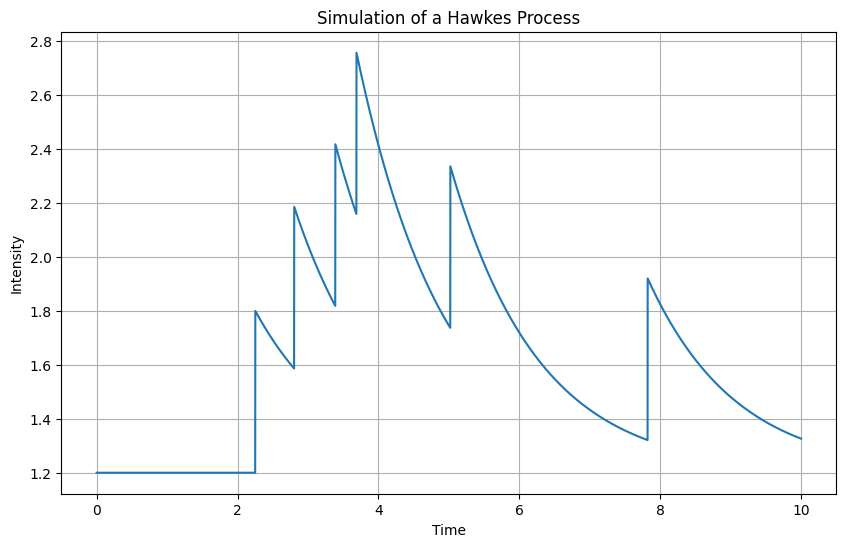
\includegraphics[width=0.6\linewidth]{figures/hawkes_process.png}
\label{fig:hawkes_process}
\end{figure}
\end{block}
\end{frame}


\begin{frame}
    \frametitle{Présentation théorique des Processus de Hawkes}
    \framesubtitle{Interprétation de la forme du modèle}

    \begin{block}{Représentation mathématique}
        \[ \lambda(t) = \lambda_0 + \sum_i \alpha_i \cdot e^{-\beta_i \cdot (t - t_i)} \]

        \begin{itemize}
            \item $\lambda(t)$ : fonction d'intensité conditionnelle à l'instant $t$
            \item $\lambda_0$ : taux de base (taux d'événements en l'absence d'influence des événements passés)
            \item $\alpha_i$ : coefficient d'excitation correspondant à l'événement $i$
            \item $\beta_i$ : coefficient de décroissance correspondant à l'événement $i$
            \item $t_i$ : temps de l'événement $i$
        \end{itemize}
    \end{block}
\end{frame}


\begin{frame}
    \frametitle{Présentation théorique des Processus de Hawkes}
    \framesubtitle{Interprétation des paramètres}

    \begin{block}{Influence du paramètre $\lambda_0$ }
    \[ \lambda(t) = \lambda_0 + \sum_i \alpha_i \cdot e^{-\beta_i \cdot (t - t_i)} \]

    \begin{itemize}
            \item $\lambda(t)$ : fonction d'intensité conditionnelle à l'instant $t$
            \item $\alpha_i$ : coefficient d'excitation correspondant à l'événement $i$ fixé à 0.6
            \item $\beta_i$ : coefficient de décroissance correspondant à l'événement $i$ fixé à 0.8
            \item $t_i$ : temps de l'événement $i$
        \end{itemize}

    \end{block}
\end{frame}
\begin{frame}
    \begin{block}{$\lambda_0$ = 0.01}
    \begin{figure}[h]
        \centering
        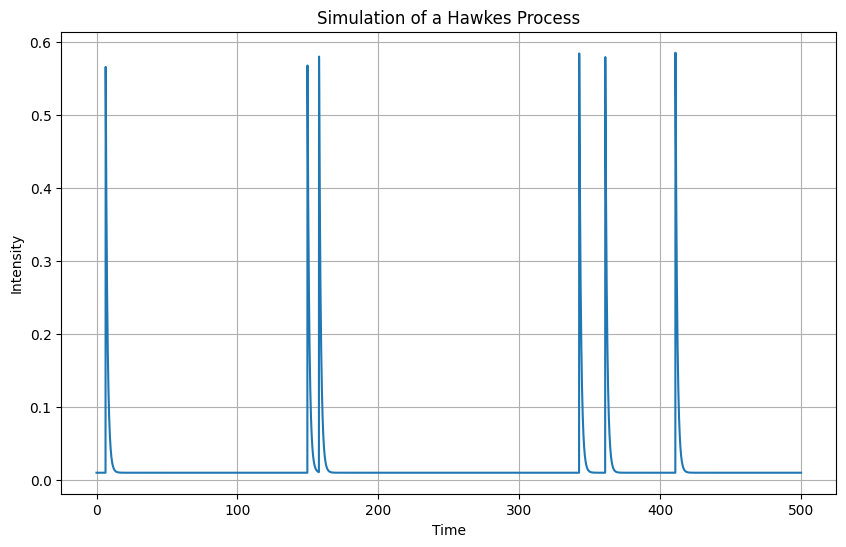
\includegraphics[width=0.6\linewidth]{figures/lamba1.png}
    \end{figure}
    \end{block}
\end{frame}

\begin{frame}
    \begin{block}{$\lambda_0$ = 0.1}
    \begin{figure}[h]
        \centering
        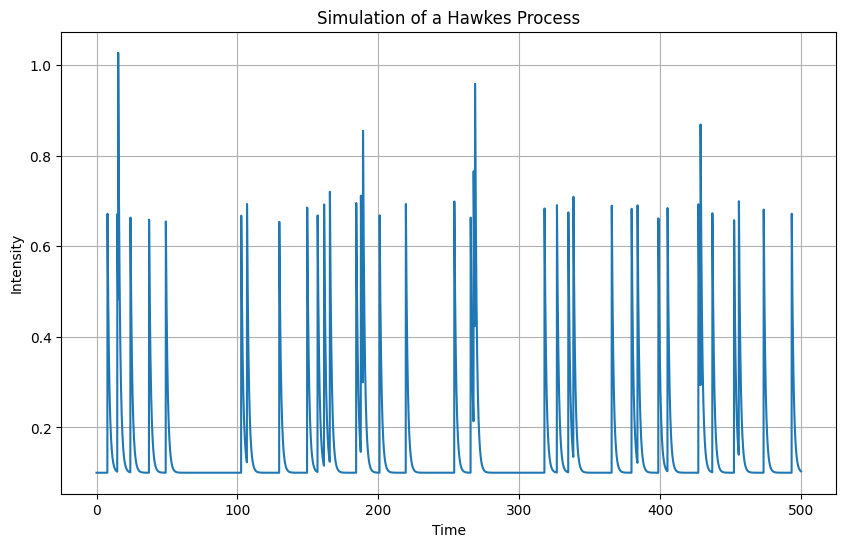
\includegraphics[width=0.6\linewidth]{figures/lambda2.png}
    \end{figure}
    \end{block}
\end{frame}

\begin{frame}
    \begin{block}{$\lambda_0$ = 1}
    \begin{figure}[h]
        \centering
        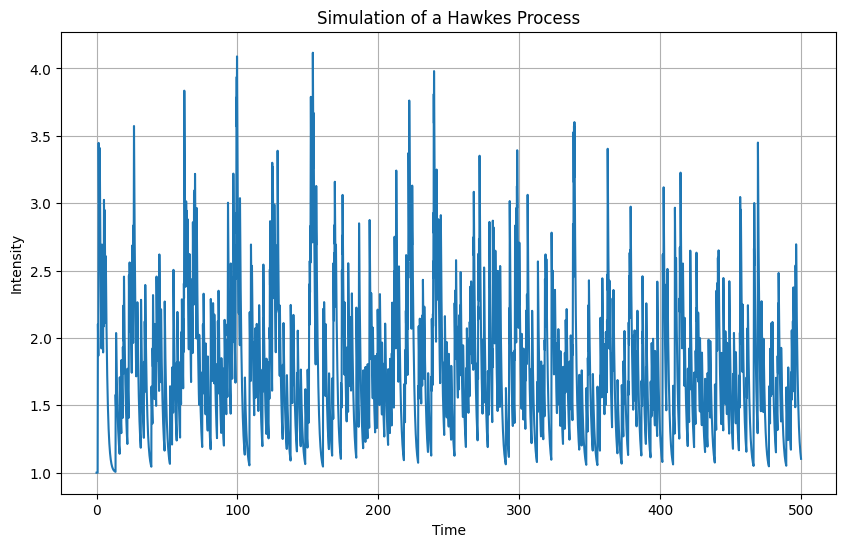
\includegraphics[width=0.6\linewidth]{figures/lambda3.png}
    \end{figure}
    \end{block}
\end{frame}

\begin{frame}
    \frametitle{Présentation théorique des Processus de Hawkes}
    \framesubtitle{Interprétation des paramètres}

    \begin{block}{Influence du paramètre $\alpha$ }
    \[ \lambda(t) = \lambda_0 + \sum_i \alpha_i \cdot e^{-\beta_i \cdot (t - t_i)} \]

    \begin{itemize}
            \item $\lambda(t)$ : fonction d'intensité conditionnelle à l'instant $t$
            \item $\lambda_0$ : taux de base (taux d'événements en l'absence d'influence des événements passés) fixé à 0.1
            \item $\beta_i$ : coefficient de décroissance correspondant à l'événement $i$ fixé à 1.2
            \item $t_i$ : temps de l'événement $i$
        \end{itemize}

    \end{block}
\end{frame}
\begin{frame}
    \begin{block}{$\alpha$ = 0.01}
    \begin{figure}[h]
        \centering
        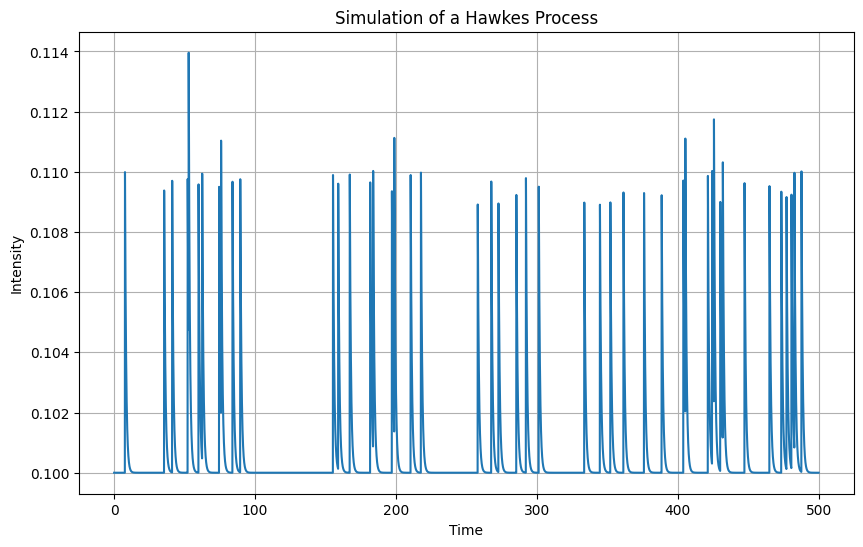
\includegraphics[width=0.6\linewidth]{figures/alpha1.png}
    \end{figure}
    \end{block}
\end{frame}

\begin{frame}
    \begin{block}{$\alpha$ = 0.1}
    \begin{figure}[h]
        \centering
        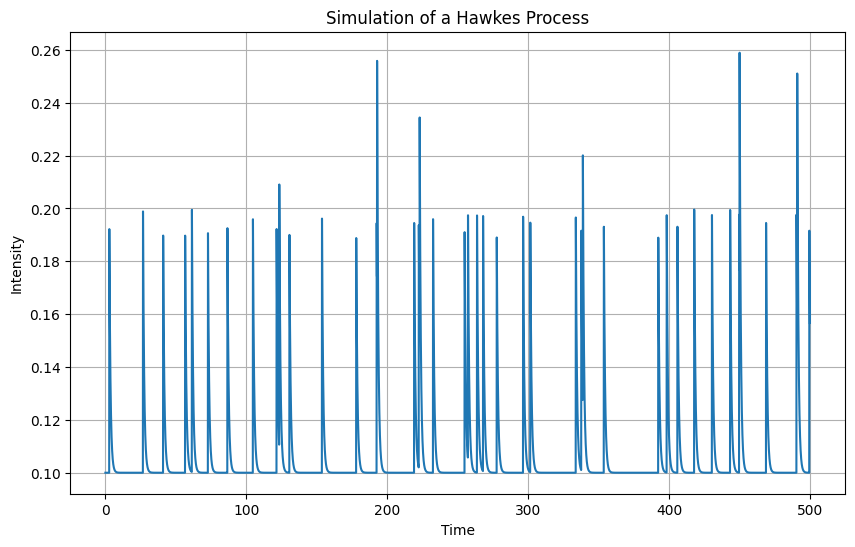
\includegraphics[width=0.6\linewidth]{figures/alpha2.png}
    \end{figure}
    \end{block}
\end{frame}

\begin{frame}
    \begin{block}{$\alpha$ = 1}
    \begin{figure}[h]
        \centering
        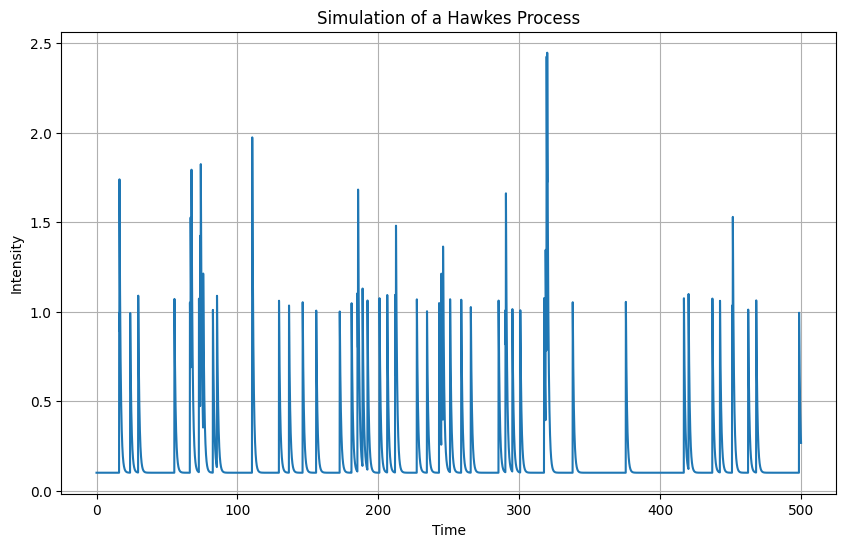
\includegraphics[width=0.6\linewidth]{figures/alpha3.png}
    \end{figure}
    \end{block}
\end{frame}

\begin{frame}
    \frametitle{Présentation théorique des Processus de Hawkes}
    \framesubtitle{Interprétation des paramètres}

    \begin{block}{Influence du paramètre $\beta$ }
    \[ \lambda(t) = \lambda_0 + \sum_i \alpha_i \cdot e^{-\beta_i \cdot (t - t_i)} \]

    \begin{itemize}
            \item $\lambda(t)$ : fonction d'intensité conditionnelle à l'instant $t$
            \item $\lambda_0$ : taux de base (taux d'événements en l'absence d'influence des événements passés) fixé à 0.1
            \item $\alpha_i$ : coefficient d'excitation correspondant à l'événement $i$ fixé à 0.6
            \item $t_i$ : temps de l'événement $i$
        \end{itemize}

    \end{block}
\end{frame}
\begin{frame}
    \begin{block}{$\beta$ = 0.05}
    \begin{figure}[h]
        \centering
        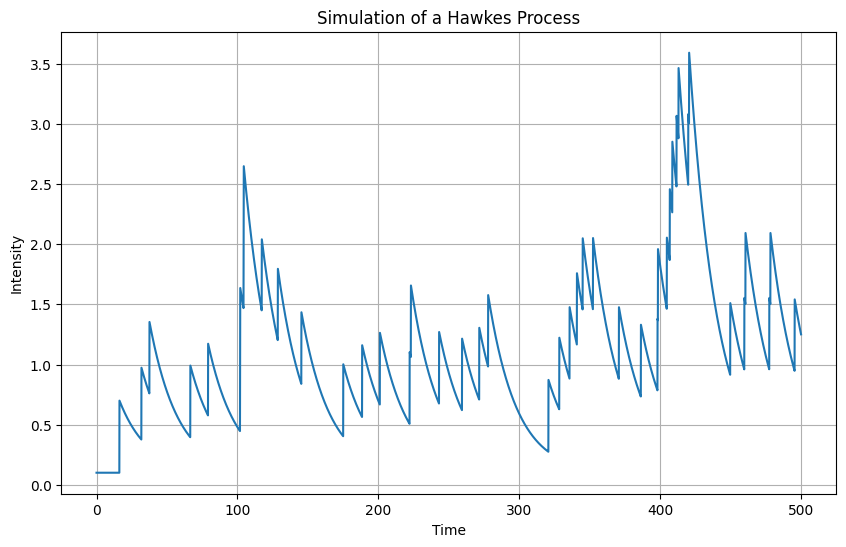
\includegraphics[width=0.6\linewidth]{figures/beta1.png}
    \end{figure}
    \end{block}
\end{frame}

\begin{frame}
    \begin{block}{$\beta$ = 0.5}
    \begin{figure}[h]
        \centering
        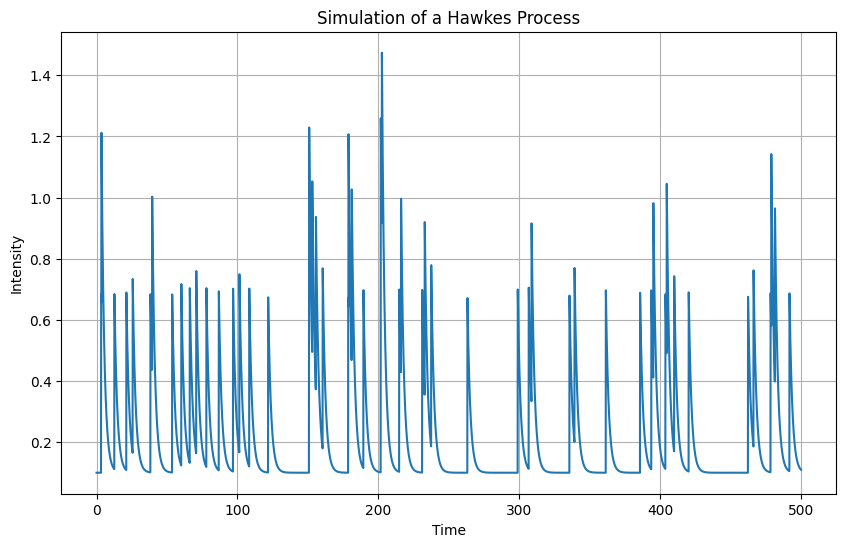
\includegraphics[width=0.6\linewidth]{figures/beta2.png}
    \end{figure}
    \end{block}
\end{frame}

\begin{frame}
    \begin{block}{$\beta$ = 5}
    \begin{figure}[h]
        \centering
        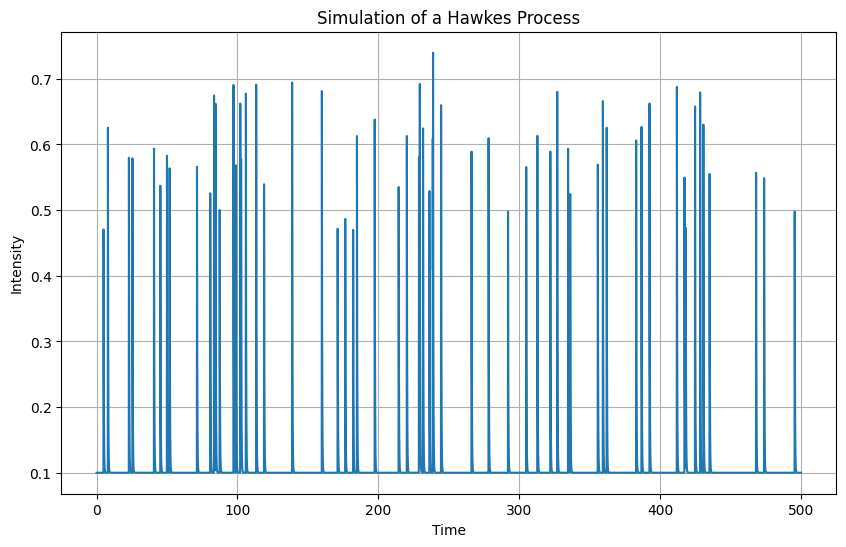
\includegraphics[width=0.6\linewidth]{figures/beta3.png}
    \end{figure}
    \end{block}
\end{frame}

\begin{frame}
    \frametitle{Présentation théorique des Processus de Hawkes}
    \framesubtitle{Simulation d'un processus de Hawkes}

    \begin{block}{Algorithme d'Ogata}
        L'algorithme d'Ogata (1981) génère des temps de survenance suivant un processus de Hawkes sur un intervalle de temps [0,T] en utilisant les paramètres $\lambda_0$, $\alpha$ et $\beta$, ainsi que la fonction d'intensité $\lambda$ qui dépend de ces trois paramètres.
    \end{block}
\end{frame}


\begin{frame}
    \frametitle{Présentation théorique des Processus de Hawkes}
    \framesubtitle{Estimation des paramètres}

    \begin{block}{Méthode du maximum de vraissemblance}
    La méthode du maximum de log-vraisemblance (ML pour Maximum Likelihood) est une technique statistique couramment utilisée pour estimer les paramètres d'un modèle statistique. L'idée est de trouver les paramètres du modèle qui maximisent la fonction de log-vraisemblance.

    \end{block}
\end{frame}

\begin{frame}
    \frametitle{Présentation théorique des Processus de Hawkes}
    \framesubtitle{Estimation des paramètres}
        \begin{figure}[h]
            \centering
            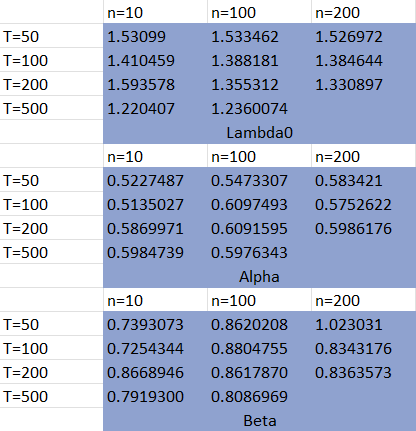
\includegraphics[width=0.5\linewidth]{figures/estim.png}
        \end{figure}
\end{frame}






